% !TEX root = ../../main.tex
\section{\acl{AD} Tools}%
\label{sec:related.ad}

As discussed in \cref{sec:intro.ad}, \ac{AD} tools have been integrated into
several modern \ac{CAD} and \ac{BIM} applications; tools that use \acp{TPL},
\acp{VPL}, or even a mixture of both approaches.

Other tools, like OpenJSCAD and ImplicitCAD, are standalone \ac{CAD} software
hosted on the web.  Being cloud-based is advantageous in many fronts: it is
inherently portable, removes the additional typical installation steps required
for desktop applications.  Alas, being relatively new, they are lacking features
in comparison to the immense feature-set of applications such as AutoCAD\@.

\Cref{tab:related.ad.summary} succinctly summarizes a list of \ac{CAD} software
that includes the capability of designing resorting to the usage of a
programming language, as well as other \ac{AD} software and tools that live
detached from existing software.  From there, Dynamo and Grasshopper are further
comparatively discussed, being relatively similar tools, however integrated
within \ac{CAD}/\ac{BIM} software designed for performing different specific
tasks.  Moreover, both include \ac{TPL} and \ac{VPL} support in different forms.

\begin{table}[htb]
  \caption[Table of programmatic CAD/BIM and AD software]{%
    \ac{CAD}/\ac{BIM} software with programmatic capabilities and \ac{AD}
    software/tools.  Added notes per tool shortly outline deemed significant
    characteristics.}\label{tab:related.ad.summary}
  \begin{tabularx}{\textwidth}{*{4}{c}X}
    \toprule
    \textbf{Application}
    & \textbf{Tool} 
    & \textbf{TPL}
    & \textbf{VPL} 
    & \textbf{Note}
    \\\midrule
    \multirow{5}{*}{AutoCAD~\cite{Autodesk:1982:AutoCAD}}
    & \multirow{2}{*}{.NET \acs{API}\label{acro:API}}
    & \multirow{2}{*}{\checkmark}
    & \multirow{2}{*}{\xmark}
    & \multirow{2}{*}{\parbox{\linewidth}{
      Powerful, but very verbose; C\# \& VB.NET}}\\ &&&&
      \\\cmidrule{2-5}
    & \multirow{2}{*}{\parbox{7em}{\centering ActiveX Automation}}
    & \multirow{2}{*}{\checkmark}
    & \multirow{2}{*}{\xmark}
    & \multirow{2}{*}{\parbox{\linewidth}{
      Deprecated, bundled separately; \acs{VBA}\label{acro:VBA}}}\\ &&&&
      \\\cmidrule{2-5}
    & Visual LISP
    & \checkmark{}
    & \xmark{}
    & \acs{IDE}\label{acro:IDE}; AutoLISP extension
    \\\midrule
    Dynamo Studio
    & \multirow{2}{*}{Dynamo~\cite{Keough:2012:Dynamo}}
    & \multirow{2}{*}{\checkmark}
    & \multirow{2}{*}{\checkmark}
    & \multirow{2}{*}{\parbox{\linewidth}{
      Data flow paradigm; Associative programming support through
      DesignScript}}
    \\\cmidrule{1-1}
    Revit~\cite{RevitTechCorp:2002:Revit} &&&&
    \\\midrule
    ArchiCAD~\cite{Graphisoft:2018:ArchiCAD}
    & \multirow{2}{*}{Grasshopper~\cite{Rutten:2018:Grasshopper}}
    & \multirow{2}{*}{\checkmark}
    & \multirow{2}{*}{\checkmark}
    & \multirow{2}{*}{\parbox{\linewidth}{
      Data flow paradigm; Rhino \acs{SDK} access, C\# \& VB.NET}}
    \\\cmidrule{1-1}
    \multirow{4}{*}{Rhinoceros3D~\cite{McNeel:2018:Rhinoceros3D}} &&&&
      \\\cmidrule{2-5}
    & \multirow{2}{*}{Python Scripting} & \multirow{2}{*}{\checkmark}
    & \multirow{2}{*}{\xmark}
    & \multirow{2}{*}{\parbox{\linewidth}{%
      Simple language; Create custom Grasshopper components}}\\ &&&&
      \\\cmidrule{2-5}
    & RhinoScript
    & \checkmark{}
    & \xmark{}
    & VBScript based
    \\\midrule
    \multirow{5}{*}{\texttt{Standalone$^\dag$}}
    & ImplicitCAD~\cite{Longtin:2018:ImplicitCAD}
    & \checkmark{}
    & \xmark{}
    & Web hosted; OpenSCAD inspired
      \\\cmidrule{2-5}
    & OpenJSCAD~\cite{Mueller:2019:OpenJSCAD}
    & \checkmark{}
    & \xmark{}
    & Web hosted; JavaScript
      \\\cmidrule{2-5}
    & OpenSCAD~\cite{Kintel:2019:OpenSCAD}
    & \checkmark{}
    & \xmark{}
    & Solid 3D models; Simple \acs{DSL}\label{acro:DSL}
      \\\cmidrule{2-5}
    & \multirow{2}{*}{Rosetta~\cite{Leitao:2011:PGDCAD}}
    & \multirow{2}{*}{\checkmark}
    & \multirow{2}{*}{\xmark}
    & \multirow{2}{*}{\parbox{\linewidth}{%
      Portable tool; Multiple front- and back-end support}}\\ &&&&
    \\\bottomrule
  \end{tabularx}

  {\scriptsize
  $^\dag$These tools are standalone software, i.e., not directly integrated into
  any specific \ac{CAD} application.
  }
\end{table}

\subsection{Dynamo}%
\label{sec:related.ad.dynamo}

An open source \ac{AD} tool available as a plug-in for Revit or by itself within
Dynamo Studio, Dynamo extends \ac{BIM} with the data and logic environment of a
graphical algorithm editor~\cite{Keough:2012:Dynamo}.  Dynamo can be used
through both a \ac{VPL} and a \ac{TPL}, showcased in
\cref{fig:related.ad.dynamo.node2code}.

\begin{figure}[htb]
  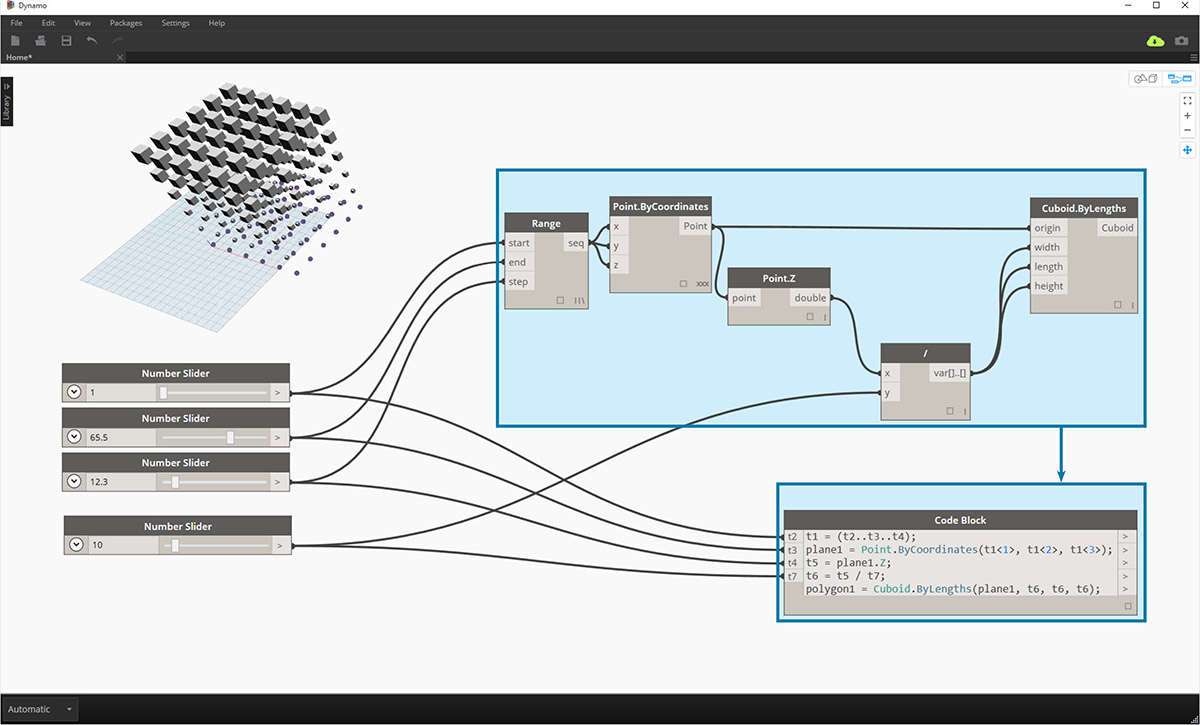
\includegraphics[width=\textwidth]{fig/dynamo-node-to-code}\\
  {\scriptsize
  Source: \url{http://primer.dynamobim.org/en/07_Code-Block/7-2_Design-Script-syntax.html}
  (Jan 2019)
  }
  \caption[Dynamo's visual interface with node to code translation]{
    Showcase of Dynamo's visual interface containing a workflow that produces
    the model on the top left.  The figure also shows Dynamo's capability of
    converting a workflow into a single DesignScript code block.}%
  \label{fig:related.ad.dynamo.node2code}
\end{figure}

In its visual form, Dynamo offers a wide variety of functions, called nodes,
most of them capable of generating an even wider variety of geometry through
node combination, wiring one's outputs to another's inputs, and resorting to
predefined mutable parameters which can serve as some of the nodes' initial
inputs.  The workflow itself is the final product: a visual program, usually
designed to execute a specific task.  Dynamo further allows extension through the
creation of custom nodes which can be shared as packages.

One of the nodes in Dynamo, aptly named code block, allows the usage of a
\ac{TPL}; a language called DesignScript.  Originally developed my Robert
Aish~\cite{Aish:2011:DesignScript}, DesignScript is a multi-paradigm
domain-specific language and is the programming language at the core of Dynamo
itself.  So much so that entire workflows can be reduced to one code block (see
\cref{fig:related.ad.dynamo.node2code}).

DesignScript is an associative language, which maintains a graph of dependencies
with variables.  Executing a script will effectively propagate the variables'
values accordingly.  By default, code blocks in Dynamo follow an associative
paradigm.  The user can, however, switch to an imperative paradigm approach
instead effortlessly if needed.

This \textit{change-propagation} mechanism in DesignScript, consequently present
in Dynamo, makes Dynamo a great tool for dealing with constraints.  However,
most users might not fully exercise DesignScript's associative capabilities and
instead approach the problem with the mindset of an imperative programming
paradigm given its overwhelming presence in and adoption by major well-known
\acp{TPL}.

\subsection{Grasshopper}%
\label{sec:related.ad.grasshopper}

Grasshopper is a graphical algorithm editor tightly integrated with
Rhinoceros3D, destined for designers who are exploring generative
algorithms~\cite{Rutten:2018:Grasshopper}.  In spite of tight integration with
Rhino, a \ac{CAD} application, it is possible to use Grasshopper along with
ArchiCAD~\cite{Graphisoft:2018:ArchiCAD,Graphisoft:2018:RGACAD}, a \ac{BIM}
tool.  \Cref{fig:related.ad.grasshopper.islamic-pattern} shows a simple example
of a Grasshopper workflow.

\begin{figure}[htb]
  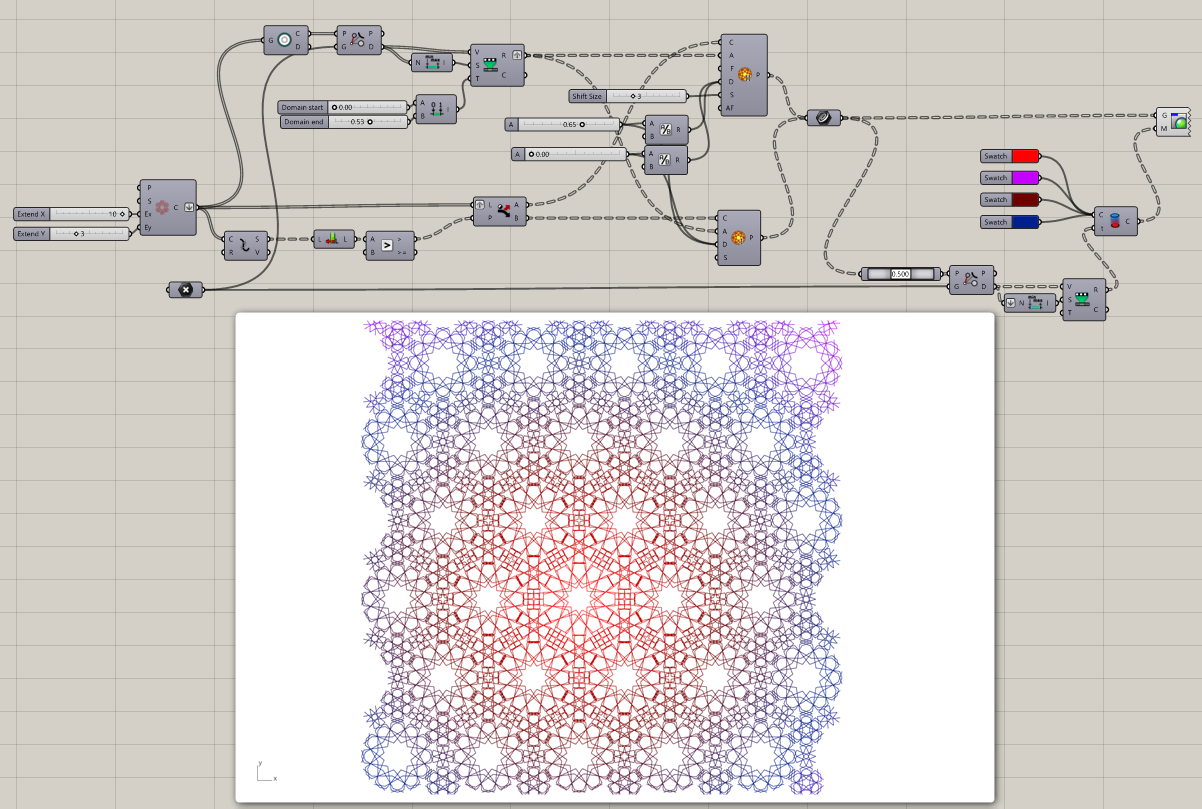
\includegraphics[width=\textwidth]{fig/grasshopper-islamic-pattern}\\
  {\scriptsize
  Source: \url{https://www.grasshopper3d.com/photo/islamic-pattern-parakeet}
  (Jan 2019)
  }
  \caption[Islamic Pattern in Grasshopper using Parakeet]{
    Islamic Pattern, by Esmaeil Mottaghi.  On top is the Grasshopper workflow to
    produce the pattern below it, aided by
    Parakeet~\cite{Esmaeil:2018:Parakeet}.}%
  \label{fig:related.ad.grasshopper.islamic-pattern}
\end{figure}

It is a closed-source product, designed by David Rutten and developed by McNeel
and Associates, Rhino's developers.  Its \ac{VPL} is as simple to use as
Dynamo's, which is crucial for users who are not familiar with programming using
a \ac{TPL}.  Nonetheless, it offers a \ac{TPL} alternative by way of custom
programmatic components.  Using C\# or VB.NET, the user can create custom code
components with access to Rhino's \ac{SDK} and
openNURBS~\cite{Lear:2018:openNURBS} within Rhino.  Alternatively, through
GhPython~\cite{Giulio:2017:GhPython}, the user can also write Python code.
Unlike DesignScript, Python and the~.NET languages don't support an associative
programming model.

Functions in Grasshopper are called components and work just like Dynamo's
nodes; a wide variety of them exist, most of them capable of producing geometry,
and they are composable, generating a workflow destined to accomplish a specific
task.
